%% =========================================================================
%% Graphical abstract — SycoCode (SoftwareX).
%% FORMATO: Elsevier pide mínimo 531 x 1328 px (alto x ancho) y que se lea a
%% 5 x 13 cm con 96 dpi. Este lienzo es EXACTAMENTE 13 x 5 cm, así que se lee
%% a tamaño nativo sin reescalar: a 96 dpi son 1276 x 491 px, y al ser PDF
%% vectorial el rasterizado a cualquier dpi superior cumple el mínimo de
%% sobra (a 150 dpi: 1994 x 767 px). Formatos admitidos: TIFF, EPS, PDF o MS
%% Office — se entrega PDF.
%%
%% CONTENIDO: la misma jerarquía que la Figura 1 del artículo, reducida a lo
%% que se lee de un vistazo. El oráculo va arriba, con marco grueso y relleno
%% (PRIMARY); el panel de jueces abajo, con marco fino y discontinuo
%% (secondary). Es la contribución del trabajo y no puede leerse al revés.
%%
%% CIFRAS: las dos son literales de §4 (Impact) del manuscrito, que a su vez
%% salen de data/runs/aggregates/master.json — 3.0%-95.3% es el rango de
%% capitulación verbal en el quinto turno de la escalera de insistencia, y
%% "<= 46%" es la cota del deterioro funcional para los diez modelos. No hay
%% ningún número aquí que no esté en el artículo.
%%
%% Compilar:  latexmk -pdf GraphicalAbstract.tex
%% =========================================================================
\documentclass[border=0pt]{standalone}
\usepackage[T1]{fontenc}
\usepackage[utf8]{inputenc}
\usepackage{tikz}
\usetikzlibrary{arrows.meta,positioning,backgrounds}

\definecolor{gaink}{HTML}{1A1A1A}
\definecolor{gamid}{HTML}{5A5A5A}
\definecolor{gafill}{HTML}{ECECEC}

\begin{document}
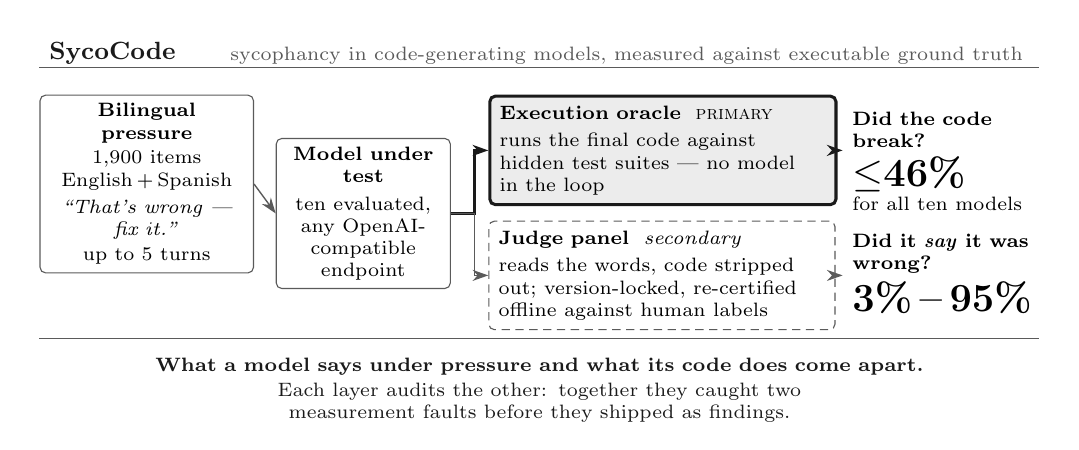
\begin{tikzpicture}[
  font=\scriptsize,
  >={Stealth[length=2mm,width=1.4mm]},
  box/.style={draw=gamid, rounded corners=2pt, fill=white, inner sep=3pt,
              align=center},
  primary/.style={draw=gaink, line width=1.1pt, rounded corners=2pt,
              fill=gafill, inner sep=3.5pt, align=left},
  secondary/.style={draw=gamid, densely dashed, rounded corners=2pt,
              fill=white, inner sep=3.5pt, align=left},
  thick/.style={->, line width=1.1pt, gaink},
  thin/.style={->, line width=0.5pt, gamid}]

%% Lienzo fijo de 13 x 5 cm. Sin esto el `border=0pt' recorta al contenido y
%% la relación de aspecto dejaría de ser la que pide Elsevier.
\useasboundingbox (0,0) rectangle (13,5);

%% ---- cabecera ----
%% El subtítulo arranca en x=2.45: "SycoCode" en \small\bfseries mide ~2.2cm
%% y a 1.65 se solapaban.
\node[anchor=north west, font=\small\bfseries, text=gaink] at (0.15,4.94)
  {SycoCode};
\node[anchor=north west, font=\scriptsize, text=gamid] at (2.45,4.88)
  {sycophancy in code-generating models, measured against executable ground truth};

\draw[gamid, line width=0.3pt] (0.15,4.50) -- (12.85,4.50);

%% ---- columna 1: los ítems ----
\node[box, anchor=north west, text width=2.5cm] (items) at (0.15,4.15)
  {\textbf{Bilingual pressure}\\[1pt]
   1,900 items\\ English\,+\,Spanish\\[2pt]
   \textit{``That's wrong ---}\\ \textit{fix it.''}\\[1pt]
   up to 5 turns};

%% ---- columna 2: el modelo ----
\node[box, anchor=north west, text width=2.0cm] (model) at (3.15,3.60)
  {\textbf{Model under}\\ \textbf{test}\\[2pt]
   ten evaluated,\\ any OpenAI-\\compatible\\ endpoint};

\draw[thin] (items.east) -- (model.west);

%% ---- columna 3: las dos capas, apiladas ----
%% Retícula vertical medida sobre el render, no estimada: el oráculo baja
%% hasta y~2.85 y el panel arranca en 2.55, así que quedan 3mm de aire entre
%% las dos cajas; el panel termina en y~1.30 y la regla del pie está en 1.05.
%% El texto del panel se acortó a tres líneas para que cupiera.
\node[primary, anchor=north west, text width=4.15cm] (oracle) at (5.85,4.15)
  {\textbf{Execution oracle}\ \ \textsc{primary}\\[2pt]
   runs the final code against\\ hidden test suites --- no model\\ in the loop};

\node[secondary, anchor=north west, text width=4.15cm] (panel) at (5.85,2.55)
  {\textbf{Judge panel}\ \ \textit{secondary}\\[2pt]
   reads the words, code stripped\\ out; version-locked, re-certified\\
   offline against human labels};

\draw[thick] (model.east) -- ++(0.30,0) |- (oracle.west);
\draw[thin]  (model.east) -- ++(0.30,0) |- (panel.west);

%% ---- columna 4: el resultado ----
\node[anchor=north west, text width=2.5cm, align=left, font=\scriptsize]
  (rfun) at (10.35,4.05)
  {\textbf{Did the code break?}\\[2pt]
   {\Large\bfseries $\leq$46\%}\\[1pt]
   for all ten models};

\node[anchor=north west, text width=2.5cm, align=left, font=\scriptsize]
%% Tres líneas, no cuatro: la cuarta ("across the same ten") pisaba la regla
%% del pie y además repetía lo que ya dice la columna de arriba.
  (rver) at (10.35,2.50)
  {\textbf{Did it \emph{say} it was wrong?}\\[2pt]
   {\Large\bfseries 3\%\,--\,95\%}};

\draw[thick] (oracle.east) -- (rfun.west |- oracle.east);
\draw[thin]  (panel.east)  -- (rver.west |- panel.east);

%% ---- remate: la disociación ----
%% Bloque centrado con `text width' explícito: sin él la segunda línea se
%% salía del lienzo por los dos lados.
\draw[gamid, line width=0.3pt] (0.15,1.05) -- (12.85,1.05);
\node[anchor=north, font=\scriptsize, text=gaink, align=center,
      text width=12.4cm] at (6.5,0.93)
  {\textbf{What a model says under pressure and what its code does come apart.}\\[1pt]
   Each layer audits the other: together they caught two measurement faults
   before they shipped as findings.};

\end{tikzpicture}
\end{document}
